

\chapter{Overview dell'architettura e delle componenti utilizzate}
\setlength{\parskip}{1em}
\setlength{\parindent}{0em}
\renewcommand{\baselinestretch}{1.15}

\label{ch:1}

\section{Obbiettivo da ottenere}

In una collaborazione tra il Dipartimento di Ingegneria dell'Informazione e l'azienda \textbf{Esse-ti S.R.L.} ci \`e stato esposto un progetto che consiste nel:

%todo non mi piace come sta messo
\begin{itemize}
    \item fornire a dei clienti un router 4G, su cui possono essere connessi vari dispositivi, ad es. di tipo domotico.
    \item rendere questi dispositivi accessibili ai clienti attraverso internet 
\end{itemize}

\begin{figure}[ht]
	\centering
	\includesvg[width=250px]{immagini/goal}
	\caption{Schema concettuale dell'obbiettivo da raggiungere}

	%TODO manca label \label{fig:modello_a_strati}
	
\end{figure}

Data la presenza del CG-NAT si vede subito che non \`e realizzabile a meno che il cliente non abbia un'IP pubblico e la sua macchina venga configurata opportunamente. Questo per\`o non \`e possibile nel caso generale, quindi per risolvere efficacemente questa topologia si deve necessariamente introdurre una terza macchina provvista di IP pubblico e che funga da ponte tra il 4G.Router e il cliente.

\begin{figure}[ht]
	\centering
	\includesvg[width=250px]{immagini/real}
	\caption{Schema concettuale dell'architettura che si dovr\`a implementare}

	%TODO manca label \label{fig:modello_a_strati}
	
\end{figure}

%todo rivedi frase
In questo modo si pu\`o configurare una VPN sul server OVH e connettervi sia il 4G.Router che la macchina del cliente. In questo modo l'unica configurazione che il cliente dovr\`a fare \`e l'installazione di un cliente VPN, ci\`o \`e il minimo possibile di configurazione.

La configurazione virtuale vista dal 4G.Router e dai clienti sar\`a quindi:

\begin{figure}[ht]
	\centering
	\includesvg[width=250px]{immagini/virtual}
	\caption{Topologia virtuale}

	%TODO manca label \label{fig:modello_a_strati}
	
\end{figure}


\section{Specifiche dei componenti}

i componenti necessari sono:

\begin{itemize}
	\item Esse-ti 4G.Router
	\item Server
	\item Host domotico
	\item Macchina del cliente
\end{itemize}

vediamo le caratteristiche minime che i componenti dovranno avere:

\subsubsection{Esse-ti 4G.Router}

Ci \`e stato fornito dall'azienda Esse-ti, consiste in un gateway 4G con funzionalità di router


\begin{figure}[ht]
	\centering
	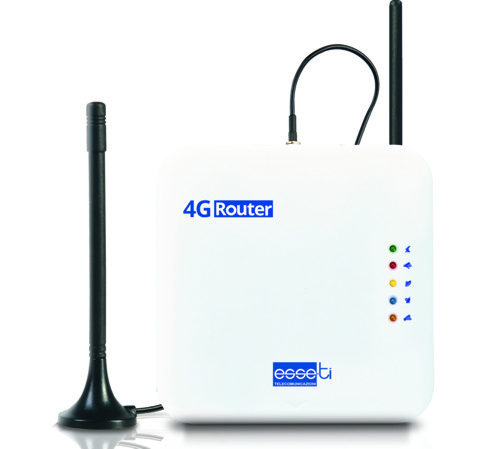
\includegraphics[width=250px]{immagini/4grouter.jpg}
	\caption{4G.Router}

	%TODO manca label \label{fig:modello_a_strati}
	
\end{figure}

Presenta 2 interfacce di rete, una radiomobile 4G, e una Wi-Fi / LAN.
Ha come sistema operativo una versione custom di OpenWrt.

\subsubsection{VPS OVHCloud}

Come server \`e stata scelta una VPS del provider OVHCloud.
Ospita il server OpenVPN.

\subsubsection{Host domotico}

Per i vari test \`e stata usata una Raspberry pi come host del router 4G.

\subsubsection{Macchina del cliente}

Deve poter essere una qualunque macchina, non ha vincoli di sistema operativo